
\documentclass[12pt]{article}

%\usepackage{fontspec}
%\setmainfont{Times New Roman}

\usepackage{tocbibind}
\usepackage{amsfonts}
\usepackage[a4paper]{geometry}
\geometry{top=2.54cm, bottom=2.54cm, left=2.54cm, right=2.54cm}

\usepackage[spanish]{babel}
\usepackage[utf8]{inputenc}
\usepackage[T1]{fontenc}
\usepackage{float}

\usepackage{graphicx} % graficos
\graphicspath{ {./contenido/images} }
\usepackage{setspace}%interlineado agrega:
% \doublespacing \onehalfspace \singlespace \spacing{x}
\spacing{1.5}

\usepackage{color}
\definecolor{AzulClaro}{rgb}{0.8,0.85,1}
\definecolor{RojoClaro}{rgb}{1,0.85,0.8}
\usepackage{amsmath}
\usepackage{array}
\usepackage{csquotes}
\usepackage[bookmarks = true, colorlinks=true, linkcolor = black, citecolor = black, menucolor = black, urlcolor = black]{hyperref}

%****************************************************
%     secciones con formato especifico

\newcommand{\comillas}[1]{``#1"}
\newcommand\ddfrac[2]{\frac{\displaystyle #1}{\displaystyle #2}}

\begin{document}


\tableofcontents


\section{General}



\subsection{Fracciones}

una fracción, número fraccionario, o numero \textbf{racional} ,
es la expresión de una cantidad dividida entre otra cantidad;
es decir que representa un cociente no efectuado de 2 números.
Las fracciones, como se observan en la imagen \nameref{Fracción}, comunes se componen de:
numerador, denominador y línea divisora
entre ambos (barra horizontal u oblicua). En una fracción común  a/b el
denominador "b" expresa la cantidad de partes iguales que
representan la unidad y \textbf{no puede ser 0} , y el numerador "a" indica
cuántas de ellas se toman.

    \begin{figure}[htb]
		\centering
        \caption{Fracción}
		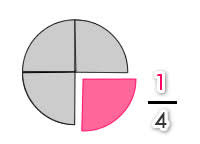
\includegraphics[ width= 5cm ]{fraccion.jpeg}
		\label{Fracción}
	\end{figure}


El conjunto matemático que contiene a las fracciones de la forma a/b, donde a y
b son números enteros y b $\not =$ 0 es el conjunto de los números racionales, denotado
como $\mathbb{Q}$.

Toda fracción es una división y toda división es una fracción. Debido a eso una
división se puede convertir en una fracción para ser simplificada.

Las fracciones pueden ser representadas como $num\div denom$, $num\/denom$ o
$\frac{num}{denom}$  en una operación matemática.



\subsubsection{Operaciones con fracciones}

    Dado que las fracciones, el conjunto $\mathbb{Q}$,  son una extensión de
    los números previamente estudiados (conjuntos $\mathbb{N}$ y $\mathbb{Z}$),
    se pueden realizar las mismas operaciones, es decir, \nameref{simplificación},
    \nameref{suma},\nameref{comparación},
    \nameref{multiplicación}, \nameref{división},
    \nameref{potenciación} y \nameref{radicalización}.


\subsubsection*{simplificación}\label{simplificación}
    Simplificar una fracción consiste en reducir tanto el numerador como el
    denominador en iguales proporciones hasta llevarlo a su mínima expresión.
    Para esto, se deben descomponer en su base y simplificar, eliminar, los números
    que sean iguales en numerador y denominador. Ejemplo:
    $$ \frac{21}{9} = \frac{factores(21)}{factores{9}} = \frac{7\times \colorbox{RojoClaro}{3} }{\colorbox{RojoClaro}{3}\times3} = \frac{7}{3}  $$
    $$ \frac{154}{22} = \frac{factores(154)}{factores{22}} = \frac{\colorbox{RojoClaro}{2}\times7\times\colorbox{RojoClaro}{11}}{\colorbox{RojoClaro}{2}\times\colorbox{RojoClaro}{11}} = \frac{7}{1}=7  $$
    $$ \frac{6}{8} = \frac{factores(6)}{factores{8}} = \frac{\colorbox{RojoClaro}{2}\times3}{\colorbox{RojoClaro}{2}\times2\times2} = \frac{3}{4}  $$

    Los 0 a la izquierda se pueden eliminar dividiendo entre 10 tantas veces sea posible:
    $$ \frac{10}{200} = \frac{1\times\colorbox{RojoClaro}{10}}{2\times\colorbox{RojoClaro}{10}\times10} = \frac{1}{20}  $$


\subsubsection*{Suma y Resta}\label{suma}

    La suma y la resta entre fracciones puede dividirse en 2 posibilidades:

    \begin{itemize}
        \item Los denominadores son \textbf{iguales}
            En este caso, se deja el mismo denominador y se suman o restan,
            dependiendo del signo y la operación, los
            numeradores. Se emplean las mismas reglas con respecto a los signos. Ejemplos:

            \textbf{Suma de fracciones}
            $$\frac{7}{5} + \frac{19}{5} = \frac{7+19}{5} = \frac{26}{5}$$

            \textbf{Resta de fracciones}
            $$\frac{7}{5} - \frac{19}{5} = \frac{7-19}{5} = \frac{-12}{5}$$
            \textbf{Recordemos} que cuando se restan números pueden haber
            resultados negativos.

            \textbf{Suma de fracciones (signos distintos)}
            $$ \frac{10}{9} + \frac{-8}{9} = \frac{10 + (-8)}{9}  = \frac{2}{9}$$
            \textbf{Cabe resaltar} que siempre hay que tener en cuenta los signos.

            \textbf{Suma algebraica, varias funciones}
            $$\frac{7}{8} + \frac{-5}{8} - \frac{-9}{8} + \frac{10}{8} =
            \frac{7+(-5)-(-9)+10}{8} = \frac{21}{8} $$

        \item Los denominadores son \textbf{diferentes}
            Cuando esto pasa, hay que llevar las fracciones a un denominador común,
            para de esta forma aplicar lo que ya vimos. Esto se puede hacer de
            2 formas, consiguiendo el \textbf{mínimo común múltiplo (mcm)} o
            haciendo una operación \comillas{cruzada} y luego multiplicamos el
            numerador por el mismo numero que multiplicamos el denominador de
            esa fracción. Ejemplos:

            \textbf{Suma de fracciones con distinto denominador}

            \textbf{mcm:}
            \begin{align*}
                &\frac{5}{3} + \frac{10}{9}\\
                &buscamos\ el\ M.C.M:\\
                &M.C.M(3) = 3\  \&\  M.C.M(9) = 3^2 \Rightarrow M.C.M(3;9) = 3^2\\
                &\frac{5\times3}{3\times3} + \frac{10\times1}{9\times1} = \frac{5\times3+10}{9} = \frac{25}{9}
            \end{align*}

            \textbf{cruzado:}
            En este método se multiplican directamente los denominadores para
            crear el nuevo denominador y luego se multiplican los  numeradores por
            los denominadores opuestos.
            \begin{align*}
                &\frac{5}{3} + \frac{10}{9}\\
                &numerador\ 1 = \frac{5}{3} \searrow \frac{10}{9} = 5\times9 = 45\\
                &numerador\ 2 = \frac{5}{3}  \nearrow \frac{10}{9} = 3\times10 = 30\\
                &denominador = \frac{5}{3} \rightarrow \frac{10}{9} = 3\times9 = 27\\
                &\frac{5\times9}{3\times9} + \frac{10\times3}{9\times3} = \frac{45+30}{27} = \frac{75}{27}
            \end{align*}

            \textbf{Nota:} aunque las fracciones se vean diferentes, tienen el mismo
            valor, a estas se les conoce como \textbf{fracciones equivalentes}
            y se puede comprobar fácilmente al ver que $25\times3=75$ y $3\times9=27$.
    \end{itemize}

\subsubsection*{Comparación}\label{comparación}

    Para comparar 2 fracciones se de deben tomar en cuenta tanto el numerador como
    el denominador. Primero se debe asegurar que el denominador sea el mismo y
    luego comparar los numeradores. Para esto se puede usar cualquiera de los
    métodos vistos en la suma (M.C.M o cruzado).

    La forma mas rápida de hacerlo es con el método de el \textbf{cruzado} de
    la suma, dado que solo hay que conseguir los numeradores, ya que estos métodos
    (también aplica con el M.C.M) aseguran un denominador  común. Ejemplo:
        \begin{align*}
            &\frac{5}{3}\ ;\ \frac{10}{9}\\
            &numerador\ 1 = \frac{5}{3} \searrow \frac{10}{9} = 5\times9 = 45\\
            &numerador\ 2 = \frac{5}{3}  \nearrow \frac{10}{9} = 3\times10 = 30\\
            &\Rightarrow como\ 45>30\ \frac{5}{3} > \frac{10}{9}
        \end{align*}



\subsubsection*{Multiplicación}\label{multiplicación}
    La multiplicación se hace de forma lineal, es decir, se
    multiplican los numeradores para obtener el numerador y los denominadores
    para obtener el denominador. Ejemplos:

    \textbf{Multiplicación}
    $$\frac{7}{5} \times \frac{6}{11} = \frac{7\times6}{5\times11} =\frac{42}{55} $$
    $$\frac{5}{3} \times \frac{10}{9} = \frac{5\times10}{3\times9} =\frac{50}{27} $$

\subsubsection*{División}\label{división}
    La división se puede hacer de dos formas:

    \textbf{Invirtiendo el denominador}

    en este caso, se invierte la fracción del denominador (el numerador pasa a
    ser el denominador y el denominador al numerador) y se multiplica por esta.
    Ejemplos:

    $$\frac{7}{5}\div \frac{6}{11} = \frac{7}{5} \times \frac{11}{6} = \frac{7\times11}{5\times6} =\frac{77}{30} $$
    $$\frac{5}{3} \times \frac{10}{9} = \frac{5}{3} \times \frac{9}{10} = \frac{5\times9}{3 \times10} =\frac{45}{30} $$

    \textbf{Doble C}

    Se coloca el denominador debajo del numerador de forma que queden 4 números
    verticales, los extremos se multiplican para dar el numerador y los internos
    se multiplican y dan como resultado el denominador. Ejemplos:

    $$\frac{7}{5}\div \frac{6}{11} =
    \ddfrac{\frac{\colorbox{AzulClaro}{7}}{\colorbox{RojoClaro}{5}}}{\frac{\colorbox{RojoClaro}{6}}{\colorbox{AzulClaro}{11}}}
    =\frac{\colorbox{AzulClaro}{$7\times11$}}{\colorbox{RojoClaro}{$5\times6$}} =\frac{77}{30} $$

    $$\frac{5}{3} \times \frac{10}{9}=
    \ddfrac{\frac{\colorbox{AzulClaro}{5}}{\colorbox{RojoClaro}{3}}}{\frac{\colorbox{RojoClaro}{10}}{\colorbox{AzulClaro}{9}}}
    = \frac{\colorbox{AzulClaro}{$5\times9$}}{\colorbox{RojoClaro}{$3\times10$}} =\frac{45}{30} $$



\subsubsection*{Potenciación}\label{potenciación}
    Una fracción puede tener potencia en su numerador, denominador, ambos o un
    exponente común para ambos. En el caso de que sea en el numerador o denominador,
    se resuelve como se acostumbra.
    Si la potenciación se aplica a ambos elementos, esta se puede dividir,
    es decir la potencia
    de una fracción es igual a la potencia del numerador entre la del denominador
    y con estos se procede de la misma forma que para los conjuntos previamente
    estudiados, y tienen las mismas propiedades. Ejemplos:

    \textbf{Potencia en el numerador}
    $$\frac{5^3}{9} = \frac{5\times5\times5}{9} =\frac{125}{9} $$

    \textbf{Potencia en el denominador}
    $$\frac{5}{3^4} = \frac{5}{3\times3\times3\times3} =\frac{5}{81} $$

    \textbf{Potencias distintas en numerador y denominador}
    $$\frac{5^3}{3^4} = \frac{5\times5\times5}{3\times3\times3\times3} = \frac{125}{81} $$

    \textbf{Potencia afectando a numerador y a denominador}
    $$ \left(\frac{4}{3}\right)^2 =  \frac{4^2}{3^2} = \frac{16}{9} $$


    \textbf{Hay que resaltar} que la operación opuesta puede realizarse también,
    es decir, si el numerador y el denominador tienen la misma potencia, se puede
    colocar una única potencia que afecte a toda la fracción.

    $$\frac{2^3}{5^3} = \left(\frac{2}{5}\right)^3 $$
    $$\frac{2^{4\times2}}{5^{3\times2}} =  \left(\frac{2^4}{5^3}\right)^2 $$


\subsubsection*{Radicalización (Raíces)}\label{radicalización}
    Una fracción puede contener radicales en su numerador, denominador, ambos o
    una raíz en común para  ambos, y se procede de la misma forma que con la potencia
    pero siendo este caso una raíz.
    Si el denominador contiene radicales, puede ser de gran ayuda \textbf{racionalizar}
    estos, especialmente si se van a realizar operaciones, tales como la
    adición o la comparación de una fracción con otra. Es también conveniente
    si la división tiene que realizarse explícitamente.
    Para racionalizar necesitamos elevar la raíz al mismo termino que esta (2
    si es cuadrada, 3 si es cubica, etc), esto se consigue al multiplicar tanto el
    numerador como el denominador por la raíz que se quiera eliminar, tantas veces
    como sea necesario (como ya hay 1, seria 1 si es cuadrática, 2 si es cubica, etc).
    ejemplos:

    \textbf{Nota:} una raíz puede ser expresada como una potencia fraccionaria,
    de esta forma se pueden facilitar cálculos.
    $\displaystyle \sqrt{a} = a^{\frac{1}{2}},\  \sqrt[3]{a} = a^{\frac{1}{3}},\ \cdots,\ \sqrt[n]{a}=a^{\frac{1}{n}}$


    \textbf{Raíz en el numerador}
    $$\frac{\sqrt{9}}{5} = \frac{3}{5} $$

    \textbf{Raíz en el denominador}
    $$\frac{5}{\sqrt{4}} = \frac{5}{2} $$

    \textbf{Raíz distintas en numerador y denominador}
    $$\frac{\sqrt[3]{27}}{\sqrt{4}}  = \frac{3}{2} $$

    \textbf{Raíz afectando a numerador y a denominador}
    $$ \sqrt{\frac{4}{25}} =  \frac{\sqrt{4}}{\sqrt{25}} = \frac{2}{5} $$

    \textbf{Racionalización}

    $$\frac{3}{\sqrt{7}} =\frac{3}{\sqrt{7}} \frac{\sqrt{7}}{\sqrt{7}}
    = \frac{3\times \sqrt{7}}{\sqrt{7}\times\sqrt{7}} = \frac{3\times \sqrt{7}}{7}   $$


    $$\frac{3}{\sqrt[3]{7}} =\frac{3}{\sqrt[3]{7}} \left(\frac{\sqrt[3]{7}}{\sqrt[3]{7}}\right)^2
    = \frac{3\times (\sqrt[3]{7})^2 }{\sqrt[3]{7}\times(\sqrt[3]{7})^2} = \frac{3\times (\sqrt[3]{7})^2}{7}   $$


\subsubsection*{Propiedades}
    Las propiedades de el conjunto $\mathbb{Q}$, las mismas que en $\mathbb{N}$
    y $\mathbb{Z}$, siendo estas extrapoladas a fracciones.

    \textbf{Nota: Todo numero entero puede escribirse como fracción, la forma mas
    simple es colocarle un denominador de 1}:
    \begin{align*}
        10=\frac{10}{1} \hspace*{1cm}	4431 &= \frac{4431}{1}\hspace*{1cm}	-75=\frac{-75}{1} \\
        \text{y mas general, con letras:  } A &= \frac{A}{1}\ ;\ A\in \mathbb{Z}
    \end{align*}


    Sean $\displaystyle \frac{A}{J},\ \frac{B}{K},\ \frac{C}{L}$ fracciones cualquiera.

\begin{itemize}
    \item \textbf{Propiedad Conmutativa} Tanto para la suma como la
        multiplicación se cumple que:

        \textbf{Aditiva:}
        $$\frac{A}{J} +\frac{B}{K} = \frac{B}{K} +\frac{A}{J}$$

        $$ \frac{3}{2} +\frac{1}{5} = \frac{17}{10} = \frac{1}{5} +\frac{3}{2}$$

        \textbf{Multiplicativa:}
        $$ \frac{A}{J} \times\frac{B}{K} = \frac{B}{K} \times\frac{A}{J}$$

        $$ \frac{3}{2} \times\frac{1}{5} = \frac{3}{10} = \frac{1}{5} \times\frac{3}{2}$$

    \item \textbf{Propiedad Asociativa} Tanto para la suma como la
        multiplicación se cumple que:

        \textbf{Aditiva:}
        $$ \frac{A}{J}+\left(\frac{B}{K}+\frac{C}{L}\right)=\left(\frac{A}{J}+\frac{B}{K}\right)+\frac{C}{L}$$

        \begin{align*}
            \frac{5}{3} +\left(\frac{1}{8} +\frac{7}{6}\right) &=\left( \frac{5}{3} +\frac{1}{8}\right) +\frac{7}{6}\\
            \frac{5}{3} +\frac{1\times6+7\times8}{8\times6} &= \frac{5\times8+1\times3}{3\times8}+\frac{7}{6}\\
            \frac{5}{3} + \frac{62}{48} &= \frac{43}{24} +\frac{7}{6} \\
            \frac{5\times48+62\times3}{48\times3} &= \frac{43\times6+7\times24}{24\times6} \\
            \frac{426}{144} &= \frac{426}{144}
        \end{align*}

        \textbf{Multiplicativa:}
        $$\frac{A}{J}\times\left(\frac{B}{K}\times\frac{C}{L}\right)=\left(\frac{A}{J}\times\frac{B}{K}\right)\times\frac{C}{L} $$

        \begin{align*}
            \frac{5}{3}\times \left(\frac{1}{8}\times \frac{7}{6}\right)  &=\left( \frac{5}{3}\times \frac{1}{8}\right)\times \frac{7}{6}\\
            \frac{5}{3} \times \frac{1\times7}{8\times6} &= \frac{1\times5}{8\times3} \times \frac{7}{6} \\
            \frac{5}{3} \times \frac{7}{48} &= \frac{5}{24} \times  \frac{7}{6} \\
            \frac{5\times7}{3\times48} &= \frac{5\times 7}{24\times6} \\
            \frac{35}{144} &= \frac{35}{144}
        \end{align*}

    \item \textbf{Propiedad distributiva} se cumple que:

        $$\frac{A}{J}\times\left(\frac{B}{K}+\frac{C}{L}\right)=\left(\frac{A}{J}\times\frac{B}{K}\right)+\left(\frac{A}{J}\times\frac{C}{L}\right) $$
        \begin{align*}
            \frac{1}{7}\times\left(\frac{2}{3}+\frac{4}{5}\right)&=\left(\frac{1}{7}\times\frac{2}{3}\right)+\left(\frac{1}{7}\times\frac{4}{5}\right)\\
            \frac{1}{7} \times \frac{2\times5+4\times3}{3\times5} &= \left(\frac{1\times2}{7\times3} \right)+\left(\frac{1\times4}{7\times5} \right) \\
            \frac{1}{7} \times  \frac{22}{15} &= \frac{2}{21} + \frac{4}{35} \\
            \frac{1\times22}{7\times15} &= \frac{2\times35+4\times21}{21\times35} \\
            \frac{22}{105} &= \frac{154}{735} \\
        \end{align*}
        aunque los resultados parezcan diferentes, se puede observar que son
        \textbf{fracciones equivalentes} ya que $$22\times7=154$$ y $$105\times7=735$$

    \item \textbf{Elemento neutro de la suma} Este sigue siento el numero 0, ya
        que al sumarlo queda igual.

        $$\frac{A}{J} + 0 = \frac{A}{J}$$

        $$\frac{57}{3} + 0 = \frac{57}{3}$$


    \item \textbf{Elemento neutro de la multiplicación} Este es el 1 ya que cualquier
        numero multiplicado por 1 sigue siendo el mismo

        $$\frac{A}{J} \times 1 = \frac{A}{J}$$

        $$\frac{28}{9} \times 1 = \frac{28}{9}$$

\end{itemize}


\subsubsection*{Fracciones Equivalentes}
    Como se ha observado, una fracción representa una cantidad especifica.
    Y por ende, las fracciones equivalentes son aquellas que expresan el mismo
    número, o cantidad, aunque el numerador y denominador de estas sean distintas.
    Esto es posible ya que, si se multiplica, o divide, el numerador y denominador de una
    fracción por el mismo numero, se obtiene una nueva forma de describir la
    misma cantidad original. \textbf{(esto es ya que al multiplicar el numerador y el
    denominador por una misma cantidad, es equivalente a multiplicarlo por 1)}
    $5\div5 = 1,\ 485\div485 = 1, -4684\div-4684 = 1 \rightarrow n\div n=1$
    Ejemplos:


        $$\frac{3}{5} =\frac{3\times4}{5\times4} = \frac{12}{20} $$
        $$\frac{-95}{3} = \frac{-95\times2}{3\times2} =\frac{190}{6} $$
        $$\frac{451}{9} = \frac{451\times3}{9\times3} =	\frac{1353}{27} $$
        $$\vdots$$
        $$\frac{A}{B} = \frac{A\times N}{B\times N}\ ;\ con \{A,B,N \} \in \mathbb{Z}$$

    \textbf{Por lo tanto,} para conseguir una fracción equivalente solo hace falta
    multiplicar el numerador y el denominador, de la función dada, por un numero cualquiera.



\subsubsection*{Fracción Generatriz}
    La fracción generatriz es aquella que da como resultado un número decimal,
    ya sea exacto o periódico, mediante una fracción irreducible, es decir,
    donde el numerador y el denominador no tienen divisores en común, de manera
    que la fracción no se puede simplificar en números más pequeños. Para
    encontrar la fracción generatriz de una expresión en particular se debe
    distinguir en 3 casos:

    \begin{itemize}
        \item \textbf{el numero es decimal exacto.} Tomamos el número sin la
            coma decimal y lo dividimos entre diez elevado al número de
            decimales, y luego simplificamos la fracción. Ejemplos:
            $$0,46 = \frac{46}{10^2}=\frac{46}{100}=\frac{ \colorbox{RojoClaro}{2}\times 23}{50\times \colorbox{RojoClaro}{2}}  \frac{23}{50} $$
            $$1,125 = \frac{1125}{10^3}=\frac{1125}{1000}=\frac{3^2\times\colorbox{RojoClaro}{$5^3$}}{2^3\times\colorbox{RojoClaro}{$5^3$}}=\frac{9}{8} $$
            $$2,4=\frac{24}{10}= \frac{3\times2\times2\times \colorbox{RojoClaro}{2}}{5\times \colorbox{RojoClaro}{2}} = \frac{12}{5}$$


        \item \textbf{El numero es periódico puro.}  Tomamos el número sin la coma
            decimal, usando una única vez el periodo, y le restamos la parte
            entera. Luego, al resultado lo dividimos entre un número que tenga
            tantos nueves como cifras tiene el periodo, y finalmente
            simplificamos hasta hallar la fracción irreductible.
            $$1,\widehat{5} =\frac{15-1}{9} =\frac{14}{9} $$
            $$ 4,\widehat{789}=\frac{4789-4}{999} =\frac{4785}{999}=\frac{1595\times \colorbox{RojoClaro}{3}}{333\times \colorbox{RojoClaro}{3}} = \frac{1595}{333} $$
            $$ 11,\widehat{45}=\frac{1145-11}{99}=\frac{1134}{99}=\frac{2\times \colorbox{RojoClaro}{$3^4$}\times7}{ \colorbox{RojoClaro}{$3^2$}\times 11} =\frac{2\times3^2\times7}{11} =\frac{126}{11}$$

        \item \textbf{El numero es periódico mixto.} Tomamos el número, sin la coma
            decimal y repitiendo el periodo solo una vez.
            A este le restamos el numero formado por la parte entera y la no periódica.
            Dividimos el resultado entre tantos 9 como el periodo y tantos 0 como
            la parte decimal.
            $$1,2\widehat{31} = \frac{1231-12}{990}= \frac{1219}{990} $$
            $$31,42\widehat{5}=\frac{31425-3142}{900} =\frac{28283}{900} $$
            $$0.4\widehat{243}=\frac{4243-4}{9990}=\frac{4239}{9990} =\frac{157\times \colorbox{RojoClaro}{$3^3$}}{2\times5\times37\times \colorbox{RojoClaro}{$3^3$}}= \frac{157}{2\times5\times37}= \frac{157}{370} $$
    \end{itemize}




\textbf{Cabe resaltar que:} de manera más general, se puede extender el
concepto de fracción a un cociente
cualquiera de expresiones matemáticas (no necesariamente números), dando origen a
funciones, ecuaciones y, permitiendo de esta forma, modelar todo tipo de
fenómenos físicos.



\newpage
\subsection{Notación Científica}
    La notación científica es una forma de escribir números muy grandes o muy pequeños
    de forma mas sencilla y eficiente. Para esto, se utilizan las propiedades de
    la potenciación, y que si se multiplica por una potencia de 10 se mueve la
    coma decimal, si la potencia de 10 es $>0$ se mueve hacia la derecha, y si
    es $<0$, se mueve hacia la izquierda.

    La idea de la notación científica es escribir el numero resultante de forma
    \textbf{Normalizada}, es decir con un numero distinto de 0 como unidad, luego
    la coma decimal, el resto de números en el mismo orden que se encontraban (si
    a partir de un punto solo quedan 0 a la derecha no se colocan), y luego
    \comillas{$\times10^{exp}$} donde \comillas{exp} seria el numero de veces que
    se corrió la coma.


\subsubsection*{De numero a notación científica}
    se quiere llevar desde un numero sin potencia hacia la forma
    $unidad, decimales \times10^{exp}$. Para esto se debe:

    \begin{enumerate}
        \item Conseguir el dígito mas significativo ya que este sera la nueva unidad,
            único dígito de la parte entera,
            este es el dígito mas a la izquierda que sea distinto de 0. Ejemplos:
            \begin{align*}
                235,39\ MSD&= 2\\
                0,12\ MSD&=1
                \\0,00000924\ MSD&=9
                \\ -4500000\ MSD &=4\\
                1507800,2\ MSD &=1
            \end{align*}



        \item Conseguir el signo, este es el mismo que el del numero.

        \item Conseguir la nueva parte decimal. Esta esta conformada por todos
            los dígitos a la derecha del MSD, este se consiguió en el paso 1.
            Cabe resaltar que si estos son todos 0, o a partir de cierto punto todos
            los números hacia la derecha son 0, se omitirán. Ejemplos:

            \begin{align*}
                235,39\ decimal= &3539\\ 0,12\ decimal=&2\\
                  0,00000924\ decimal=&24\\ -4500000\ decimal=&5\\1507800,2\ decimal=&5078002
            \end{align*}

        \item Calcular el exponente. Esta compuesto en 2 partes, el signo y el
            valor.
            \begin{itemize}
                \item El signo sera:
                    \begin{itemize}
                        \item + si el MSD esta a la izquierda de la coma \comillas{,}

                        \item - si el MSD esta a la derecha de la coma \comillas{,}
                    \end{itemize}
                \item El valor sera: la cantidad de espacios, números, que se tiene
                    que correr el MSD hasta llegar a ser el único dígito a la izquierda
                    de la coma \comillas{,}
            \end{itemize}
            Ejemplos:
            \begin{align*}
                2 \colorbox{RojoClaro}{35},39\ exp=&+2\\  \colorbox{RojoClaro}{0},12\ exp=&-1\\
                 \colorbox{RojoClaro}{0,000\ 00}924\ exp=&-6\\ -4 \colorbox{RojoClaro}{500\ 000}\ exp=&+6\\1 \colorbox{RojoClaro}{507800},2\ exp=&+6
            \end{align*}




    \end{enumerate}
    Finalmente:
        $$235,39=2,3539 \times10^{2}$$
        $$0,12 = 1,2 \times10^{-1}$$
        $$0,000\ 009\ 24 = 9,24 \times10^{-6}$$
        $$-4\ 500\ 000 = -4,5 \times10^{6}$$
        $$1\ 507\ 800,2 = 1,507\ 800\ 2 \times10^{6}$$


\subsubsection*{de notación científica a numero}
    se quiere llevar desde la forma $unidad, decimales \times10^{exp}$ hacia un
    numero sin potencia. Para esto se debe correr la coma tantas veces lo diga
    el exponente y de acuerdo al signo, si es positivo( +, $exp>0$) hacia la derecha, si es
    negativo (-, $exp<0$) hacia la izquierda. Cuando no hay mas elementos a la derecha
    o izquierda(respectivamente del signo del exponente) después de la coma se
    completa con 0 (ceros).

    \textbf{nota:} para ayudar a recordar hacia donde se mueve la coma, es útil
    usar el menor o mayor como la punta de una flecha, así se tiene que:
    $-5<0$ entonces hacia la izquierda y $5>0$ entonces hacia la derecha.

        $$2,3539 \times10^{2}= 2,\colorbox{RojoClaro}{35}39 = 235,39 $$
        $$1,2 \times10^{-1} = 0\colorbox{RojoClaro}{1},2 = 0,12  $$
        $$9,24 \times10^{-6}=\text{Completamos con 0 a la izquierda: } 0\colorbox{RojoClaro}{000\ 009},24 =0,000\ 009\ 24  $$
        $$-4,5 \times10^{6}=\text{Completamos con 0 a la derecha: }-4,\colorbox{RojoClaro}{500\ 000}=-4\ 500\ 000  $$
        $$1,507\ 800\ 2 \times10^{6}= 1, \colorbox{RojoClaro}{507\ 800}\ 2= 1\ 507\ 800,2  $$



    \textbf{Dato curioso:} se usan potencias de 10 ya que esta es la base del
    sistema decimal, es decir, tenemos 10 posibles opciones para la unidad
    ($\{0,1,2,3,4,5,6,7,8,9\}$, en otros sistemas se utilizan potencias de la base
    para desplazar la coma, en binario potencias de 2, hexadecimal potencias de 16,
    etc.

\newpage
\subsection{Teorema de Pitágoras}
    En matemáticas, el teorema de Pitágoras es una relación fundamental en
    geometría euclidiana entre los tres lados de un triángulo \textbf{rectángulo}.
    Este teorema se puede escribir como una ecuación que relaciona las longitudes
    de los lados a, b y c, (catetos e hipotenusa) y a menudo se le  llamada ecuación
    pitagórica y estipula que:

    \comillas{\emph{En todo triangulo rectángulo, el cuadrado de la hipotenusa es
    igual a la suma de los cuadrados de los catetos}}.

    Sean $a,\ b$ los catetos y $c$ la hipotenusa, como se observa en \ref{triangulo}:

    $$c^2 = a^2+b^2$$
    y despejando para hipotenusa y cada cateto:
    $$c= \sqrt{a^2+b^2}$$
    $$a=\sqrt{c^2-b^2}$$
    $$b= \sqrt{c^2-a^2}$$


    \begin{figure}[htb]
		\centering
        \caption{Triangulo rectángulo}
		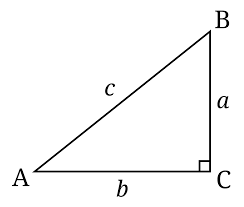
\includegraphics[ width= 5cm ]{triangulo.png}
		\label{triangulo}
	\end{figure}

    \textbf{Recordemos:} que la hipotenusa de todo triangulo es el lado mas grande
    y siempre esta opuesta al ángulo de 90°


\newpage
\subsection{Potenciación}
    La potenciación es una operación matemática entre 2 términos, \textbf{base}
    y \textbf{exponente} y se escribe de la forma: $base^{exp}$, la potenciación
    se puede aplicar a cualquier conjunto de números ($\mathbb{N}, \mathbb{Z},
    \mathbb{Q}, \mathbb{R}, \mathbb{C}$) y consiste en:

    \textbf{Multiplicar tantas veces la base como lo indique el exponente}

    Cuando el exponente es 2 se le suele que esta elevado a \textbf{cuadrado}
    y al exponente 3 se le dice elevado al \textbf{cubo} y ante exponentes mayores
    se suele leer a la cuarta, quinta, etc potencia. O el numero esta elevado a
    cuatro, cinco, etc.

    \textbf{Nota:} Cuando la base es un numero negativo, se encierra este entre
    paréntesis para evitar confusión, ya que \textbf{el signo si afecta y se
    multiplica}.

    \textbf{Es importante: } saber que todo numero elevado a 0 tiene como resultado
    1. ejemplos: $5^0=1,\ 5441^0=1,\ (-443148)^0=1,\ n^0 = 1 $, con n siendo distinto de 0.
    si la base y el exponente son ambos 0 la operación no esta definida, es decir
    $0^0$ es indeterminado, no existe.
    Ejemplos:

    \begin{align*}
        15^2 =& 15\times15 = 225\\
        6^4 =& 6\times6\times6\times6 = 1296\\
        (-8)^3 =& -8\times-8\times-8 = -512\\
        (-24)^2 =& -24\times-24= 576\\
     \end{align*}

    De los ejemplos se observa que:
    \begin{itemize}
        \item Los resultados de la potenciación crecen muy rápido, mientras
            mayor sea  el exponente, mayor sera el valor absoluto del numero resultante
            siempre que la base sea distinta de 1 o 0.
        \item todo numero elevado a 1 es el mismo numero.
        \item Si la base es 1 el resultado siempre sera 1.
        \item \textbf{Todo numero elevado a una potencia par da resultado positivo}
    \end{itemize}

    \textbf{para las fracciones}, se utiliza una propiedad de la potenciación, y se
    elevan tanto el numerador como el denominador al exponente común. Ejemplos:

    \begin{align*}
        \left(\frac{10}{8}\right)^3=& \frac{10^3}{8^3} = \frac{10\times10\times10}{8\times8\times8} = \frac{1000}{512}\\
        \left(\frac{5}{3}\right)^{2} =& \frac{5^2}{3^2}= \frac{5\times5}{3\times3} = \frac{25}{9} \\
        \left(\frac{-8}{7}\right)^{4} =& \frac{(-8)^4}{7^4}= \frac{-8\times-8\times-8\times-8}{7\times7\times7\times7} = \frac{4096}{2401} \\
        \left(\frac{a}{b}\right)^{n} =& \frac{a^n}{b^n} \frac{a\times a\times \cdots\times a}{b\times b\times \cdots\times a}
     \end{align*}

\subsubsection*{Propiedades de la potenciación}
    \subsubsection*{Potencia Par}
        Como se menciono anteriormente, \textbf{todo numero elevado a una potencia
        par da como resultado un numero positivo}, además, es bueno recordar que
        un numero par tiene la forma $2\times N$, con N $\in \mathbb{Z}$ o dicho
        de otra forma, es divisible entre 2.

        \begin{align*}
            (-8)^{4} =& -8\times-8\times-8\times-8 =& 4096\\
            9^3=& 9\times9\times9 =& 729\\
            (-864)^2  =& -864\times-864 = -746496\\
            (-1)^88 =& -1\times-1\times-1\times \cdots \times -1 = 1
        \end{align*}

    \subsubsection*{Potencia Impar}
        En este caso, todo numero elevado a potencia impar tendrá el mismo signo
        que la base. De nuevo, recordemos que un numero impar tiene la forma
        $(2\times N)+1$, es decir, no es divisible entre 2.

        \begin{align*}
            (-3)^3 =& -3\times-3\times-3 = -27\\
            (-745)^1 =& -745\\
            (-2)^{7} =& -2\times-2\times-2\times \cdots \times -2 = -128\\
            (-1)^{97} =& -1\times -1\times-1\times\cdots\times -1 = -1\\
        \end{align*}


    \subsubsection*{Exponente Negativo}
        Un exponente negativo en una potencia implica que la base es una fracción
        con numerador 1 y denominador base, como el numerador es 1 el exponente
        solo afectara en el denominador y sera un numero positivo, es decir:
        $$A^{-n}= \frac{1}{A^n} $$
        Ejemplos:

    \begin{align*}
        7^{-1} &= \frac{1}{7} \\
        5^{-4}& = \frac{1}{5^4} = \frac{1}{625} 		\\
        (-4)^{-3} &= \frac{1}{(-4)^3} = \frac{1}{64} \\
        98^{-2} &= \frac{1}{98}
        \left(\frac{3}{4} \right)^{-2} = \frac{1}{\left(\frac{3}{4} \right)^{2}} =\frac{4^2}{3^2} = \frac{16}{9}
    \end{align*}




    \subsubsection*{Multiplicación de potencias de igual base}
    Cuando se multiplican 2 o mas potencias de igual base, se deja la misma base
    y se \textbf{suman} los exponentes. Ejemplos:

    \begin{align*}
        2^{10}\times2^5 =& 2^{10+5} = 2^{15} = 32768\\
        5^2\times5^{3} =& 5^{2+3} = 5^{5} =3125\\
        9 \times 9^2 =& 9^{1+2} = 9^3 = 729 \\
        &\vdots\\
        A^m\times A^n &= A^{m+n}
    \end{align*}

    \subsubsection*{División de potencia de igual base}
    Cuando se dividen 2 o mas potencias de igual base, se deja la misma base y se
    \textbf{restan} los exponentes. Ejemplos:

    \begin{align*}
        2^{10}\div2^5 =& 2^{10-5} = 2^5 = 32\\
        5^2\div5^{2} =& 5^{2-2} = 5^{0} =1\\
        9^4 \div 9^2 =& 9^{4-2} = 9^2 = 81 \\
        &\vdots\\
        A^m\div A^n &= A^{m-n}
    \end{align*}


    \subsubsection*{Potencia de un producto}
    La potencia de un producto es igual al producto de los operandos elevados al
    exponente original, esto es
    \textbf{La potencia puede repartirse a los multiplicandos},
    $(A\times B)^{n} = A^n \times B^n $.

    Se hace especial énfasis en que es en \textbf{productos}, esto \textbf{no
    aplica ni en suma ni en restas}, en esos casos se usan \textbf{productos notables}.

    Ejemplos:

    \begin{align*}
        (3\times5)^2 =&3^2\times5^2= 9\times25=225		\\
        (10\times(-3))^3 =& 10^3 \times (-3)^3 = 1000\times(-27) = -27000\\
        (5\times4)^4 =&5^4\times4^4 = 625\times256= 160000
    \end{align*}



    \subsubsection*{potencia de un cociente}
    La potencia de un cociente es igual al cociente de los operandos elevados al
    exponente original, es decir, \textbf{La potencia puede repartirse al numerador
    y al denominador}. De nuevo se recuerda que \textbf{LA POTENCIA NO SE PUEDE
    REPARTIR EN SUMA O RESTA}, de presentarse una operación de ese estilo se
    aplica un producto notable (véase \refname{producto-notable}).

    $$ \left(\frac{A}{B}\right)^{n} = \frac{A^n}{B^n}  $$

    \begin{align*}
       \left(\frac{2}{3}\right)^{3} =& \frac{2^3}{3^3}= \frac{8}{27}	\\
        \left(\frac{7}{5}\right)^{2} =& \frac{7^2}{5^2} =\frac{49}{25} \\
        \left(\frac{8}{9}\right)^{4} =&\frac{8^4}{9^4} = \frac{4096}{6561}\\
        \left(\frac{-1}{2}\right)^{10} =& \frac{(-1)^10}{2^10} = \frac{1}{1024}
    \end{align*}

    \subsubsection*{Potencia de una potencia}
    La potencia de una potencia es igual a una nueva potencia, esta tiene como base
    la original y como exponente el producto de los dos exponentes
    de la original. De esta forma: $(B^{exp1})^{exp2} = B^{exp1\times exp2}$
    donde $B$ es la base y $exp1$, $exp2$ los exponentes.

    \begin{align*}
        \left(5^2\right)^{3} =& 5^{2\times3}= 5^6 =15625	\\
        \left(7^2\right)^{2} =& 7^{2\times2}= 7^4  =2401 \\
        \left(2^3\right)^{4} =& 2^{3\times4}=2^12  = 4096\\
        \left(\left(\frac{-1}{2}\right)^{5}\right)^2 =&\left(\frac{-1}{2}\right)^{2\times5}= \left(\frac{-1}{2}\right)^{10}=\frac{(-1)^{10}}{2^{10}} = \frac{1}{1024}
    \end{align*}

    \subsubsection*{Exponente Racional}

    Un exponente racional implica que el numero que es el exponente pertenece
    al conjunto $\mathbb{Q}$, es una fracción.
    De este tipo de expresiones es que se crearon las raíces, ya que son un
    caso particular del mismo (cuando el numerador es 1), esto significa que:
    $A^\frac{1}{den} = \sqrt[den]{A}$


    Por otro lado, el numerador actúa como un exponente normal, siendo la
    expresión general:

    $A^{\frac{num}{den} } = \sqrt[den]{A^{num}}$

    Ejemplos:

    \begin{align*}
        10^{\frac{1}{4}} &= \sqrt[4]{10} 		\\
        5^{\frac{2}{3} } &= \sqrt[3]{5^2} = \sqrt[3]{25} \\
        44^{\frac{-2}{5} }&= \frac{1}{44^{\frac{2}{5}}} = \frac{1}{ \sqrt[5]{44^2} }= \frac{1}{ \sqrt[5]{1936} } \\
        (-3)^{\frac{4}{5}} &= \sqrt[5]{(-3)^4} = \sqrt[5]{81}
    \end{align*}



    \subsubsection*{Potencia Indeterminada}
        La potencia $0^0$ es una potencia indeterminada, es decir no existe,
        para referirse a este tipo de resultados se dice que \textbf{presenta una
        forma indeterminada $0^0$}.

        \textbf{Como dato curioso: }
        Existen otras formas indeterminadas por ejemplo $\frac{0}{0}$,
        $\frac{\infty}{\infty}$ los cuales se estudian en cursos universitarios y
        superiores con \textbf{limites}.

\vspace*{1cm}

    \textbf{Cabe resaltar:} que es posible encontrarse mas de una propiedad en
    la misma potencia, y para resolverla basta con aplicar las propiedades que hagan
    falta, paso a paso.





\section{Ecuaciones}

\subsection{Inecuaciones}
\subsection{Sistema de Ecuaciones}





\section{Funciones}

\section{Funciones}


\subsection{Función Lineal}
\subsection{Función Cuadratica}
\subsection{Función Polinomica}
\subsection{Conicas}
\subsection{Función Exponencial}
\subsection{Función Logaritmica}
\subsection{Funciones Trigonometricas}





\section{Polinomios}

\subsection{Productos notables}\label{producto-notable}

\begin{itemize}
\item cuadraticos
\end{itemize}

\subsection{Factorizacion}\label{Factorización}
\subsection{Regla de Ruffini}
\subsection{Coeficientes indeterminados}
\subsection{Radicales}





\section{Vectores}

\section{Vectores}

\subsection{vectores}

 un vector es un ente matematico, es decir, es una figura creada para dar
    forma a la realidad como lo son la recta o el plano. Fue creada para
    representar fenomenos que no pueden ser descritos solamente con numeros, por
    ejemplo, la velocidad y las fuerzas. Son, por tanto, una construccion
    mas compleja que  la de los numeros y representan \textbf{una magnitud con
    direccion y sentido}. Graficamente son representados como una recta con
    cierto angulo de inclinacion y un sentido marcado por ua flechita, la
    direccion a la que apuntan.  Para poder representar un vector se necesitan
    al menos 2 puntos, el inicio del vector y el final (graficamente, si unes 2
    puntos obtienes una recta, algebraicamente se restan $punto_{final}-
    punto_{inicial}=magnitud_{vector}$ )

    Existen muchos vectores,y estos son utilizados para dar representacion a
    fenomenos fisicos. En general un vector de dimension $n$ es una tupla (un
    conjunto ordenado invariable de la forma $(x_1,x_2,\cdots,x_n)$ de numeros
    reales.

    Un vector posee 2 caracteristicas:

    \begin{itemize} \item Modulo, es su valor, la longitud del segmento o la
                cantidad de espacios que se mueve en un determinado eje (o
                ejes).

        \item Direccion, En algunos textos se descompone como direccion y
            sentido.  Es el angulo del segmento con respecto a un eje
            (normalmente x) y su sentido con respecto al origen (va o no hacia
            ese punto). Ejemplo: $29^o$ noreste sentido hacia arriba.
    \end{itemize}

    Graficamente un vector de 2 dimensiones en el origen se ve de la forma:

\begin{tikzpicture}[scale=1.6]

    \draw[style=help lines,step=0.5cm] (-4.1,-4.1)grid(4.1,4.1);

    \draw[<->] (-4.2,0)--(4.2,0) node[right]{$x$};
    \draw[<->] (0,-4.2)--(0,4.2) node[above]{$y$};
    \draw (0,0) node[anchor=north west ]{0};

    \draw[line width=2pt,blue](0,0)--(3,3.2) node[anchor=south west]{$\boldsymbol{\vec{u}}$};
    \draw[line width=2pt,red](0,0)--(-3,-3.2) node[anchor=north east]{$\boldsymbol{\vec{-u}}$};
\end{tikzpicture}

y de 3 dimensiones, en el origen se ve de la forma:


\begin{tikzpicture}[scale=1.8]
%standard tikz coordinate definition using x, y, z coords
    \coordinate (O) at (0,0,0);

\tikzset{
    x={(0:1cm)},y={(230:0.7cm)},z={(90:1cm)}
  }
 %draw a grid in the x-y plane
    \foreach \x in {-0.5,0,...,4}
        \foreach \y in {-0.5,0,...,4}
        {
            %eje xy
            \draw[very thin,red!30] (\x,-0.5) -- (\x,4.1);
            \draw[very thin,red!30] (-0.5,\y) -- (4.1,\y);
        }
%tikz-3dp %draw a grid in the x-z plane
    \foreach \x in {-0.5,0,...,4}
        \foreach \y in {0,0.5,...,4}
        {
            %eje xz
            \draw[very thin,blue!20] (\x,0,0) -- (\x,0,4.1);
            \draw[very thin,blue!20] (-0.5,0,\y) -- (4.1,0,\y);
        }
%draw axes
    \draw[->,thick] (0,0,0) -- (4.2,0,0) node[anchor=north east]{$x$};
    \draw[->,thick] (0,0,0) -- (0,4.1,0) node[anchor=north west]{$y$};
    \draw[->,thick] (0,0,0) -- (0,0,4.1) node[anchor=south]{$z$};

%draw a vector from O to P
    \draw[line width=2pt,blue!80,->] (O) -- (3,4,3.5)node[anchor=south west]{$\boldsymbol{\vec{u}}$};
    \draw[blue!80,dashed] (3,4,3.5)--(3,0,3.5);
    \draw[blue!80,dashed] (3,4,3.5)--(3,4,0);
\end{tikzpicture}




    Adicionalmente, los vectores poseen una \textbf{dimension}, esta representa
    la cantidad de coordenadas las cuales cubre. Los vectores mas usados son
    los bidimensionales, que poseen 2 coordenadas, $X,Y$ y representan el plano
    o espacio bidimensiona, son duplas ordenadas y pertenecen al espacio
    $\mathbb{R}^2$ y los tridimensionales, que utilizan 3 coordenadas $X,Y,Z$ y
    representan el espacio tridimensional perteneciendo al espacio
    $\mathbb{R}^3$.

    De igual forma, pueden utilizarse tantas dimensiones como hagan falta y el
    vector pertenecera al espacio $\mathbb{R}^n$ donde $n$ es la cantidad de
    coordenadas que posee y es un numero natural.

    Cabe destacar que estos vectores tambien son muy utilizados ya que permiten
    extrapolar fenomenos fisicos de mas variables, como por ejemplo el
    comportamiento de una caldera, o en el caso de 4 dimensiones cubrir tambien
    el tiempo $(x,y,z,t)$ y describir una fuerza o suceso en un espacio y
    tiempo determinado.

    Los vectores normalmente se utilizan para representar fuerzas, movimientos,
    variaciones, es decir cualquier condicion fisica que implica una potencia o
    cambio ejercido en una direccion particular.

    Por simplificacion, se trabajara en su mayotia con vectores en
    $\mathbb{R}^2$ y en $\mathbb{R}^3$ mas todos los conceptos son
    Extrapolables.

    Las operaciones, basicas, que se realizan con vectores son la suma
    algebraica, multiplicacion por un escalar. Adicionalmente esta definida la
    multiplicacion entre vectores como \textbf{producto punto} y
    \textbf{producto cruz}.

    \textbf{la division vectorial no esta definida!}, sin embargo, para ciertos
    tipos de vectores como fasores o numeros complejos se define una
    multiplicacion y una division especial.



    \subsubsection{Representacion}

    Los vectores pueden ser representados de 2 formas, mediante la descripcion
    individual de sus caracteristicas o mediante una magnitud y uno angulos de
    referencia. Ambas formas de representacion son equivalentes y se pueden
    llevar de una forma a otra.

    La forma de magnitud y angulo suele ser utilizada para vectores en
    $\mathbb{R}^2$ y mas especificamente en un conjunto de vectores con propiedades
    adicionales como lo son los numeros complejos, ya que es facil la
    transformacion, el producto y la division definido \textbf{unicamente para
    ellos} y para representarlos solamente se necesita un
    angulo. Para vectores de mayor dimension suele usarse la representacion por
    coordenadas, esto es debido a que para representar una linea en 3
    direcciones hacen falta al menos 2 angulos, uno de giro horizontal y otro
    vertical (a esto se le conoce como coordenadas esfericas).


    \subsubsection{Representacion en coordenadas rectangulares}

    Esta forma de representacion se basa en descomponer el vector en los
    valores asociados que poseen en cada eje. Por ejemplo, si el vector es de
    $\mathbb{R}^2$ tiene coordenadas $x$ e $y$, por lo tanto el vector puede
    ser representado como la union del origen (o un punto de referencia
    cualquiera) y los desplazamientos correspondientes en los ejes X,Y , si el
    vector es de 3 coordenadas, entonces serian X,Y,Z y asi sucesivamente. A
    este tipo de coordenadas se le conocen como \textbf{ coordenadas
    cartesianas o rectangulares}.

    De esta forma, un vector puede escribirse de 2 formas, como tupla ordenada
    o como suma de componentes, en donde cada componente va a estar indicada
    por un \textbf{vector unitario}, el cual no es mas que una letra la cual
    indica a que eje corresponde; $\hat{\imath}$ para x, $\hat{\jmath}$ para y,
    $\hat{k}$ para k.

    De esta forma, un vector puede ser escrito de la forma:

    $$\vec{v}=(v_1,v_2,v_3,\cdots,v_n),\ v_i \in \mathbb{R}$$


    o de la forma:

    $$\vec{v}=v_1\cdot\hat{\imath}+v_2\cdot\hat{\jmath}+v_3\cdot\hat{k}+\cdots$$

    Graficamente, estas composiciones son:

    Para 2 dimensiones:


\begin{tikzpicture}[scale=1.6]
    \draw[style=help lines,step=0.5cm] (-2.1,-2.1)grid(4.1,4.1);
    \draw[<->] (-2.2,0)--(4.2,0) node[right]{$x$};
    \draw[<->] (0,-2.2)--(0,4.2) node[above]{$y$};
    \draw (0,0) node[anchor=north west ]{0};

    \draw[line width=3pt,blue,->](0,0)--(3,3) node[anchor=south west]{$\boldsymbol{\vec{u}}$};


    \draw[line width=1pt,blue!80,->](0,0)--(3,0) node[anchor=south west]{$\boldsymbol{\vec{u_x}}$};
    \draw[line width=1pt,blue!80,->](0,0)--(0,3) node[anchor=south west]{$\boldsymbol{\vec{u_y}}$};

\end{tikzpicture}

    Para 3 dimensiones:


\begin{tikzpicture}[scale=1.8]
%standard tikz coordinate definition using x, y, z coords
    \coordinate (O) at (0,0,0);

\tikzset{
    x={(0:1cm)},y={(230:0.7cm)},z={(90:1cm)}
  }
 %draw a grid in the x-y plane
    \foreach \x in {-0.5,0,...,4}
        \foreach \y in {-0.5,0,...,4}
        {
            %eje xy
            \draw[very thin,red!30] (\x,-0.5) -- (\x,4.1);
            \draw[very thin,red!30] (-0.5,\y) -- (4.1,\y);
        }
%tikz-3dp %draw a grid in the x-z plane
    \foreach \x in {-0.5,0,...,4}
        \foreach \y in {0,0.5,...,4}
        {
            %eje xz
            \draw[very thin,blue!20] (\x,0,0) -- (\x,0,4.1);
            \draw[very thin,blue!20] (-0.5,0,\y) -- (4.1,0,\y);
        }
%draw axes
    \draw[->,thick] (0,0,0) -- (4.2,0,0) node[anchor=north east]{$x$};
    \draw[->,thick] (0,0,0) -- (0,4.1,0) node[anchor=north west]{$y$};
    \draw[->,thick] (0,0,0) -- (0,0,4.1) node[anchor=south]{$z$};

%draw a vector from O to P

    \draw[line width=1pt,red!80,->] (O) -- (0,4,3.5)node[anchor=south west]{$\boldsymbol{\vec{u_{yz}}}$} ;
    \draw[line width=1pt,red!80,->] (O) -- (3,0,3.5)node[anchor=south west]{$\boldsymbol{\vec{u_{xz}}}$} ;
    \draw[line width=1pt,red!80,->] (O) -- (3,4,0)node[anchor=south west]{$\boldsymbol{\vec{u_{xy}}}$} ;

    \draw[red!80,dashed] (3,4,3.5)--(3,0,3.5);
    \draw[red!80,dashed] (3,4,3.5)--(3,4,0);
    \draw[red!80,dashed] (3,4,3.5)--(0,4,3.5);

    \draw[line width=1pt,green!80,->] (O) -- (3,0,0)node[anchor=south west]{$\boldsymbol{\vec{u_{x}}}$} ;
    \draw[line width=1pt,green!80,->] (O) -- (0,4,0)node[anchor=south east]{$\boldsymbol{\vec{u_{y}}}$} ;
    \draw[line width=1pt,green!80,->] (O) -- (0,0,3.5)node[anchor=south west]{$\boldsymbol{\vec{u_{z}}}$} ;


    \draw[green!80,dashed] (3,0,3.5)--(0,0,3.5);
    \draw[green!80,dashed] (3,0,3.5)--(3,0,0);

    \draw[green!80,dashed] (0,4,3.5)--(0,4,0);
    \draw[green!80,dashed] (0,4,3.5)--(0,0,3.5);

    \draw[green!80,dashed] (3,4,0)--(3,0,0);
    \draw[green!80,dashed] (3,4,0)--(0,4,0);

    \draw[line width=2pt,blue!80,->] (O) -- (3,4,3.5)node[anchor=south west]{$\boldsymbol{\vec{u}}$} ;
\end{tikzpicture}




    Ejemplos:

    $$\vec{V}=(2,1)=2\hat{\imath}+1\hat{\jmath}$$
    $$\vec{V}=(-3,8)=-3\hat{\imath}+8\hat{\jmath}$$
    $$\vec{V}=(-21,-35)=-21\hat{\imath}-35\hat{\jmath}$$

    $$\vec{V}=(3,4,7)=3\hat{\imath}+4\hat{\jmath}+7\hat{k}$$
    $$\vec{V}=(-2,13,9)=-2\hat{\imath}+13\hat{\jmath}+9\hat{k}$$
    $$\vec{V}=(32,-4,-22)=32\hat{\imath}-4\hat{\jmath}-22\hat{k}$$


    \subsubsection{Representacion en magnitud y angulos}

    La otra forma de representar un vector es mediante una magnitud (que
    representa el tamaño del segmento-recta) y uno o mas angulos, los cuales
    son tomados con respecto a un punto de referencia y permiten orientar el
    vector en el espacio. Este tipo de coordenadas es conocido como
    \textbf{coordenadas polares} para 2 variables-ejes y \textbf{coordenadas
    esfericas} para 3 variables-ejes. Se escribe de la forma:

    $$\vec{V}= magnitud \phase{\theta} $$
    $$\vec{V}= magnitud  \phase{\theta}\phase{\phi} $$

    Donde, $magnitud$ se suele representar con la letra $r$ y los angulos
    suelen venir expresados en grados, ademas, $\theta$ mide el plano XY y
    $\phi$ el angulo con el eje Z. Y estan limitados por:


     \begin{align*}
         0\leq r&<\infty & 0\leq\theta&<2\pi & 0\leq\phi&\leq\pi \\
         0\leq r&<\infty & 0^\circ\leq\theta&<360^\circ & 0^\circ\leq\phi&\leq180^\circ
    \end{align*}

    Cabe resaltar que la nomenclatura puede variar y en algunos textos $\theta$
    se cambia por $\phi$, esto es debido a una falta de estadarizacion (como los
    cm y pulgadas, kg y libras, etc) en este texto se utilizara la convencion
    antes descrita para evitar confusiones, ya que en polares se usa $\theta$ para
    el plano XY.

    Ejemplos:


    $$\vec{V}=12 \phase{38^\circ} $$
    $$\vec{V}=23,22 \phase{98^\circ} $$
    $$\vec{V}=87,9 \phase{128^\circ} $$

    $$\vec{V}=45 \phase{12^\circ}\phase{30^\circ} $$
    $$\vec{V}=5 \phase{342^\circ}\phase{120^\circ} $$
    $$\vec{V}=23 \phase{2^\circ}\phase{180^\circ} $$

    Ambas representaciones son equivalentes,y esta equivalencia se logra
    mediante la trigonometria, mas especificamente un triangulo rectangulo.



\begin{tikzpicture}[scale=1.8]
    \draw[style=help lines,step=0.5cm] (-2.1,-2.1)grid(4.1,4.1);
    \draw[<->] (-2.2,0)--(4.2,0) node[right]{$x$};
    \draw[<->] (0,-2.2)--(0,4.2) node[above]{$y$};
    \draw (0,0) node[anchor=north west ]{0};


    \draw[line width=1pt,blue!80,->](0,0)--(3,0) node[anchor= south west]{$\boldsymbol{\vec{u_x}}$};
    \draw[line width=1pt,blue!80,->](3,0)--(3,3) node[anchor=north  west]{$\boldsymbol{\vec{u_y}}$};
    \fill[green!70] (0,0)--(1,0) node[anchor=south west]{$\theta$} -- (1,0)  arc [start angle=0,end angle=45,x radius=1, y radius=1] ;

    \draw[line width=2pt,red,->](0,0)--(3,3) node[anchor=south west]{$\boldsymbol{\vec{u}}$};
\end{tikzpicture}


\tdplotsetmaincoords{60}{110}
\begin{tikzpicture}[scale=1.8,tdplot_main_coords]
%standard tikz coordinate definition using x, y, z coords
    \coordinate (O) at (0,0,0);

\tikzset{
    x={(0:1cm)},y={(230:0.7cm)},z={(90:1cm)}
  }
 %draw a grid in the x-y plane
    \foreach \x in {-0.5,0,...,4}
        \foreach \y in {-0.5,0,...,4}
        {
            %eje xy
            \draw[very thin,red!30] (\x,-0.5) -- (\x,4.1);
            \draw[very thin,red!30] (-0.5,\y) -- (4.1,\y);
        }
%tikz-3dp %draw a grid in the x-z plane
    \foreach \x in {-0.5,0,...,4}
        \foreach \y in {0,0.5,...,4}
        {
            %eje xz
            \draw[very thin,blue!20] (\x,0,0) -- (\x,0,4.1);
            \draw[very thin,blue!20] (-0.5,0,\y) -- (4.1,0,\y);
        }
%draw axes
    \draw[->,thick] (0,0,0) -- (4.2,0,0) node[anchor=north east]{$x$};
    \draw[->,thick] (0,0,0) -- (0,4.1,0) node[anchor=north west]{$y$};
    \draw[->,thick] (0,0,0) -- (0,0,4.1) node[anchor=south]{$z$};

%draw a vector from O to P

    \draw[red!80,dashed] (3,4,3.5)--(3,4,0);

    \begin{scope}[canvas is xy plane at z=0, thick]
        \draw (1,0) arc (0:53.13:1) ;
        \draw (1,0) node[anchor=north west ]{$\theta$};
    \end{scope}

    \tdplotsetthetaplanecoords{53.13}
    \tdplotdrawarc[tdplot_rotated_coords]{(0,0,0)}{1}{0}{40.5729}{anchor=south west}{$\phi$}

    \draw[line width=1pt,red!80,->] (O) -- (3,4,0)node[anchor=south west]{$\boldsymbol{\vec{u_{xy}}}$} ;
    \draw[line width=2pt,blue!80,->] (O) -- (3,4,3.5)node[anchor=south west]{$\boldsymbol{\vec{u}}$} ;
\end{tikzpicture}


    Como se observa en la imagen, y se sabe de la representacion por
    coordenadas, un vector puede representarse como sus coordenadas en los
    ejes, estas representaciones forman los catetos del triangulo y la magnitud
    total representa la hipotenusa del mismo. De esta forma, se tiene que:

    Para 2 variables:

    polares a cartesianas
    $$\vec{V_x}= r\cdot cos(\theta)$$
    $$\vec{V_y} =  r\cdot sen(\theta)$$

    cartesianas a polares
    $$ r = \sqrt{V_x ^2+v_y^2}$$
    $$\theta= arctan\left(\frac{V_y}{V_x}\right)$$



    para3 variables:

    esfericas a cartesianas
    $$\vec{V_x}= r\cdot cos(\theta) \cdot sin(\phi)$$
    $$\vec{V_y} = r\cdot sen(\theta)\cdot sin(\phi)$$
    $$\vec{V_z}=r\cdot cos(\phi)$$

    cartesianas a esfericas
    $$ r = \sqrt{V_x ^2+v_y^2+v_z^2}$$
    $$\theta= arctan\left(\frac{V_y}{V_x}\right)$$
    $$\phi = arcos\left(\frac{V_z}{r}\right)$$


    Ejemplos:


    Transformar a polares:

     \begin{align*}
         \vec{V}&=(2,1) \\
         r &= \sqrt{2^2+1^2}  \rightarrow r= \sqrt{5} \\
         \theta&= arctan\left(\frac{1}{2}\right)  \rightarrow \theta= 26,57 ^\circ \\
    \end{align*}

     \begin{align*}
         \vec{V}&=(-3,8) \\
         r &= \sqrt{(-3)^2+8^2} \rightarrow r= \sqrt{73} \\
         \theta&= arctan\left(\frac{8}{-3}\right)  \rightarrow \theta= -69,44^\circ =-69,44^\circ+360^\circ=290.56 \\
    \end{align*}

     \begin{align*}
         \vec{V}&=(-21,-35) \\
         r &= \sqrt{(-21)^2+(-35)^2}  \rightarrow r= 7\sqrt{34} \\
         \theta&= arctan\left(\frac{-35}{-21}\right)  \rightarrow \theta= 59,04^\circ\\
    \end{align*}

    Transformar a esfericas:

    \begin{align*}
        \vec{V}&=(3,4,7) \\
        r &= \sqrt{3^2+4^2+7^2} \rightarrow w =\sqrt{74}  \\
        \theta&= arctan\left(\frac{4}{3}\right)  \rightarrow \theta= 53,13^\circ \\
        \phi &=arcos\left(\frac{7}{\sqrt{74}}\right)  \rightarrow \phi= 35,54^\circ\\
    \end{align*}

    \begin{align*}
        \vec{V}&=(-2,13,9) \\
        r &= \sqrt{(-2)^2+13^2+9^2}  \rightarrow w =\sqrt{254}  \\
        \theta&= arctan\left(\frac{13}{-2}\right)  \rightarrow \theta= -81,25^\circ= 278.75^\circ\\
        \phi &= arcos\left(\frac{9}{\sqrt{254}}\right)  \rightarrow \phi=  55,62^\circ\\
    \end{align*}

    \begin{align*}
        \vec{V}&=(32,-4,-22) \\
        r &= \sqrt{32^2+(-4)^2+22^2}  \rightarrow w =2\sqrt{381}  \\
        \theta&= arctan\left(\frac{13}{-2}\right)  \rightarrow \theta= -7,13^\circ=352,87^\circ \\
        \phi &= arcos\left(\frac{-22}{2\sqrt{381}}\right)  \rightarrow \phi= 124,3^\circ\\
    \end{align*}

    Transformar a rectangulares
    \begin{align*}
        \vec{V}&=12\phase{38^\circ}  \\
        \vec{V_x}&= 12\cdot cos(38^\circ) \rightarrow \vec{V_x} = \sqrt{9,456} \\
        \vec{V_y}& =  12\cdot sen(38^\circ)  \rightarrow \vec{V_y}= \sqrt{7,388} \\
    \end{align*}

    \begin{align*}
        \vec{V}&=23,22 \phase{98^\circ}  \\
        \vec{V_x}&= 23,22\cdot cos(98^\circ)  \rightarrow \vec{V_x} = \sqrt{18,298} \\
        \vec{V_y}& =  23,22\cdot sen(98^\circ)  \rightarrow \vec{V_y}= \sqrt{14.296} \\
    \end{align*}

    \begin{align*}
        \vec{V}&=87,9 \phase{128^\circ}  \\
        \vec{V_x}&= 87,9\cdot cos(128^\circ) \rightarrow \vec{V_x} = \sqrt{-54,117} \\
        \vec{V_y}& =  87,9\cdot sen(128^\circ)  \rightarrow \vec{V_y}= \sqrt{69.266} \\
    \end{align*}


    \begin{align*}
        \vec{V}&=45 \phase{12^\circ}\phase{30^\circ} \\
        \vec{V_x}&= 45\cdot cos(12^\circ) \cdot sin(30^\circ)  \rightarrow \vec{V_x} = \sqrt{22,008} \\
        \vec{V_y} &= 45\cdot sen(12^\circ)\cdot sin(30^\circ) \rightarrow \vec{V_x} = \sqrt{4,678} \\
        \vec{V_z}&=45\cdot cos(30^\circ)  \rightarrow \vec{V_x}= \sqrt{38,971} \\
    \end{align*}

    \begin{align*}
        \vec{V}&=5 \phase{342^\circ}\phase{120^\circ}\\
        \vec{V_x}&= 5\cdot cos(342^\circ) \cdot sin(120^\circ)   \rightarrow \vec{V_x} = \sqrt{4,118} \\
        \vec{V_y} &=5r\cdot sen(342^\circ)\cdot sin(120^\circ)  \rightarrow \vec{V_x} = \sqrt{-1,338} \\
        \vec{V_z}&=5\cdot cos(120^\circ)  \rightarrow \vec{V_x} = \sqrt{-2,5} \\
    \end{align*}

    \begin{align*}
        \vec{V}&=23 \phase{0^\circ}\phase{180^\circ}\\
        \vec{V_x}&= 23\cdot cos(2^\circ) \cdot sin(180^\circ)   \rightarrow \vec{V_x} = \sqrt{0} \\
        \vec{V_y} &= 23\cdot sen(2^\circ)\cdot sin(180^\circ)  \rightarrow \vec{V_x} = \sqrt{0} \\
        \vec{V_z}&= 23\cdot cos(180^\circ)  \rightarrow \vec{V_x} = \sqrt{-23} \\
    \end{align*}


    \subsubsection{Suma}

    La suma de vectores se realiza con los vectores en su forma cartesiana, es
    decir,\textbf{ para poder sumar 2 vectores debemos llevarlo a su forma
    rectangular}, La forma en la que se hace la suma es simplemente sumar sus
    componentes internas, es decir su representacion en $x$ con su respectivo
    par, la de $y$ con $y$ y asi sucesivamente.

    Sean $\vec{v},\vec{u}$ dos vectores cualesquiera de $\mathbb{R}^n$ tal que:

    $$\vec{v}=(v_1,v_2,v_3,\cdots,v_n)\ ; \vec{u}=(u_1,u_2,u_3,\cdots,u_n)$$
    $$\vec{r}=\vec{v+u}=(v_1+u_1,v_2+u_2,v_3+u_3,\cdots,v_n+u_n)$$

    \textbf{Recuerde que,} una suma algebraica es la suma con signo de los
    elementos, esto quiere decir que incluye a la resta ya que si se suman
    numeros de signos opuestos es lo mismo a restarlos.

    Graficamente, la forma mas sencilla es dibujar el primer vector en el
    origen y en su extremo dibujar el siguiente vector (el que se le sumara
    algebraicamente), luego se unen el origen del primer vector (corresponde
    con el origen del plano por como se definió) y el fin del segundo vector
    y este es el vector suma resultante.

    Graficamente, para $\mathbb{R}^2$:


\begin{tikzpicture}[scale=1.6]
    \draw[style=help lines,step=0.5cm] (-2.1,-2.1)grid(5.1,5.1);
    \draw[<->] (-2.2,0)--(5.2,0) node[right]{$x$};
    \draw[<->] (0,-2.2)--(0,5.2) node[above]{$y$};
    \draw (0,0) node[anchor=north west ]{0};

    \draw[line width=2pt,blue!40,->](0,0)--(2,2) node[anchor=south]{$\boldsymbol{\vec{u}}$};

    \draw[line width=2pt,red!40,->](2,2)--(4,3) node[anchor=south east ]{$\boldsymbol{\vec{v}}$};

    \draw[line width=2pt,green!40,->](0,0)--(4,3) ;
    \draw[line width=2pt,green!40] (2.3,1.7) node[anchor=west ]{$\boldsymbol{\vec{r}=\vec{u}+\vec{v}}$};
\end{tikzpicture}

    Ejemplos: Sumar los siguientes vectores

    \begin{align*}
        \vec{V}& =(2,1) \ \ ;\ \ \ \vec{U} =(-3,8)		\\
        \vec{R}&= (2-3 ,1+8 )   \rightarrow \vec{R} = (-1 ,9  )
    \end{align*}

    \begin{align*}
        \vec{V}& =(-21,-35)  \ \ ;\ \ \  \vec{U} =(-3,8)		\\
        \vec{R}&= (-21-3 ,-35+8  )  \rightarrow \vec{R} = (-24 ,-27  )
    \end{align*}

    \begin{align*}
        \vec{V}& =(-21,-35)  \ \ ;\ \ \  \vec{U} =(2,1)		\\
        \vec{R}&= (-21+2 , -35+1 )   \rightarrow \vec{R} = (-19 ,-34  )
    \end{align*}




    \begin{align*}
        \vec{V}& =(3,4,7)  \ \ ;\ \ \   \vec{U} =(-2,13,9)		\\
        \vec{R}&= (3-2 ,4+13 ,7+9 )   \rightarrow \vec{R} = (4,17,16 )
    \end{align*}

    \begin{align*}
        \vec{V}& =(3,4,7)  \ \ ;\ \ \  \vec{U} =(32,-4,-22)		\\
        \vec{R}&= (3+32, 4-4,7-22 )  & \rightarrow \vec{R} &= ( 35,0 ,-15 )
    \end{align*}

    \begin{align*}
        \vec{V}& =(-2,13,9)  \ \ ;\ \ \   \vec{U} =(32,-4,-22)		\\
        \vec{R}&= (-2+32 ,13-4 ,9-22 )  \rightarrow \vec{R} = (30, 9,-13 )
    \end{align*}


    \subsubsection{Producto por escalar}

    El producto por escalar es una operacion que toma un vector cualesquiera
    $\vec{v} \in \mathbb{R}^n$ y un escalar (numero) cualquiera $\alpha \in
    \mathbb{R}$. Consiste en multiplicar ese escalar por todos los elementos del
    vector modificando de esta forma su magnitud. Cuando el vector se encuentra
    en coordenadas polares o esfericas solamente se modifica la magnitud,
    multiplicandola por el escalar, el angulo permanece igual.

    Sean $\vec{v}$ un  vector cualesquiera de $\mathbb{R}^n$  tal que:

    $$\vec{v}=(v_1,v_2,v_3,\cdots,v_n)\ ; \alpha \in \mathbb{R} $$
    $$\vec{r}=\alpha\cdot\vec{v}=(v_1\cdot\alpha,v_2\cdot\alpha,v_3\cdot\alpha,\cdots,v_n\cdot\alpha)$$

    Graficamente:
    \begin{itemize}
        \item Aumenta su tamaño si $|\alpha| >1$.
        \item Reduce su tamaño si $|\alpha| <1$.

        \item Invierte su direccion y  sigue las reglas de la magnitud anteriores
            si $\alpha<0$.

        \item Permanece igual si $\alpha=1$.
        \item Se anula se $\alpha = 0$.
    \end{itemize}


\begin{tikzpicture}[scale=1.6]
    \draw[style=help lines,step=0.5cm] (-3.1,-3.1)grid(5.1,5.1);
    \draw[<->] (-3.2,0)--(5.2,0) node[right]{$x$};
    \draw[<->] (0,-3.2)--(0,5.2) node[above]{$y$};
    \draw (0,0) node[anchor=north west ]{0};

    \draw[line width=2pt,blue!40,->](0,0)--(4,4) ;
    \draw[line width=2pt,blue!40] (3.3,3) node[anchor=south west]{$\alpha>1$};

    \draw[line width=2pt,red,->](0,0)--(-1,-1) ;
    \draw[line width=2pt,red] (-2,-1.2) node[anchor=west ]{$\alpha<0$ y $|\alpha|<1$};

    \draw[line width=2pt,->](0,0)--(2,2) node[anchor=west]{$\alpha=1$};
\end{tikzpicture}


    Ejemplos, multiplicar los siguientes vectores por los escalares:

    \begin{align*}
        \vec{V}& =(2,1)  \ \ ;\ \ \  \alpha =3 		\\
        \vec{R}&= (2\times3,1\times3 )   \rightarrow \vec{R}= (6,3 )
    \end{align*}

    \begin{align*}
        \vec{V}& =(-3,8)  \ \ ;\ \ \  \alpha = 8		\\
        \vec{R}&= (-3 \times8,8 \times8 )   \rightarrow \vec{R}= (-24,64 )
    \end{align*}

    \begin{align*}
        \vec{V}& =(-21,-35)  \ \ ;\ \ \ \alpha = -5		\\
        \vec{R}&= (-21 \times-5,-35 \times-5)  \rightarrow \vec{R} = (105,175 )
    \end{align*}





    \begin{align*}
        \vec{V}& =(3,4,7)  \ \ ;\ \ \  \alpha= -9	\\
        \vec{R}&= (3 \times-9,4 \times-9,7 \times-9  )  \rightarrow \vec{R}= (-27,-36,-63 )
    \end{align*}

    \begin{align*}
        \vec{V}& =(-2,13,9)  \ \ ;\ \ \  \alpha = 12 		\\
        \vec{R}&= (-2 \times12, 13 \times12, 9 \times12)  \rightarrow \vec{R}= (-24,156,108)
    \end{align*}

    \begin{align*}
        \vec{V}& =(32,-4,-22)  \ \ ;\ \ \  \alpha = -1		\\
        \vec{R}&= (32 \times-1, -4 \times-1, -22 \times-1 )  \rightarrow \vec{R}= (-32,4,22)
    \end{align*}




    \subsubsection{Multiplicacion entre vectores}

    La multiplicacion entre vectores es una propiedad definida de una forma
    muy distinta a la multiplicacion numerica. Esto se debe a la complejidad de
    los vectores la cual permite defini varios tipos de multiplicaciones posibles
    las cuales tienen sentido. Las 2 Multiplicacionesmas conocidas son \textbf{
    el producto punto y el producto cruz}, ademas de esto existen otras formas
    de realizar multiplicaciones como la es la de los numeros complejos, siendo
    esta definida de tal forma que permite incluso crear una division.

    Los producto punto y producto cruz \textbf{No tienen operacion inversa} y es
    por esto que \textbf{no existe la division vectorial}.

    \subsubsection{Producto punto}

    Este tipo de multiplicacion es realizable par todos los vectores y da como
    resultado un escalar, es decir un numero.

    Se escribe de la forma: $\vec{r} = \vec{v}\cdot\vec{u}$, con
    $\vec{v},\vec{u}$ vectores cualesquiera.

    La forma de definir este producto varia, existen varios procedimientos
    equivalentes, las dos mas conocidas son con la norma de cada uno de los vectores
    y el angulo entre vectores, y el que se trabajara aca que es una suma del
    producto entre los componentes del vector. Es decir:

    Sean $\vec{v},\vec{u}$ dos vectores cualesquiera de $\mathbb{R}^n$ tal que:

    \begin{align*}
        \vec{v}&=(v_1,v_2,v_3,\cdots,v_n) \ \ ;\ \ \ \vec{u}=(u_1,u_2,u_3,\cdots,u_n)\\
        \vec{r}&=\vec{v}\cdot\vec{u}= (v_1\cdot u_1,v_2 \cdot u_2,v_3 \cdot u_3,\cdots,v_n \cdot u_n)\rightarrow
        \vec{r}= \sum_{i=0}^{n} v_i\cdot u_i
    \end{align*}


    Ejemplos:

    \begin{align*}
        \vec{V}& =(2,1) \ \ ;\ \ \  \vec{U} =(-3,8)		\\
        \vec{R}&= 2\cdot-3 +1\dot8   \rightarrow \vec{R}= 2
    \end{align*}

    \begin{align*}
        \vec{V}& =(-21,-35)  \ \ ;\ \ \  \vec{U} &=(-3,8)		\\
        \vec{R}&= -21\cdot-3 +\ -35\cdot8    \rightarrow \vec{R}= -217
    \end{align*}

    \begin{align*}
        \vec{V}& =(-21,-35)  \ \ ;\ \ \ \vec{U} &=(2,1)		\\
        \vec{R}&= -21\cdot2 + -35\cdot1   \rightarrow \vec{R}= -77
    \end{align*}




    \begin{align*}
        \vec{V}& =(3,4,7)   \ \ ;\ \ \  \vec{U} =(-2,13,9)		\\
        \vec{R}&= 3\cdot-2 +4\cdot13 +7\cdot9   \rightarrow \vec{R} = 109
    \end{align*}

    \begin{align*}
        \vec{V}& =(3,4,7)  \ \ ;\ \ \  \vec{U} =(32,-4,-22)		\\
        \vec{R}&= 3\cdot32 + 4\cdot-4 +7\cdot22    \rightarrow \vec{R} = -74
    \end{align*}

    \begin{align*}
        \vec{V}& =(-2,13,9)  \ \ ;\ \ \   \vec{U} =(32,-4,-22)		\\
        \vec{R}&= -2\cdot32 + 13\cdot-4 +9\cdot-22 )  \rightarrow \vec{R} = -314
    \end{align*}

    \subsubsection{Producto cruz}

    Este tipo de multiplicacion da como resultado un vector, graficamente, da
    como resultado un vector perpendicular al plano ($90^\circ$) formado por
    los dos vectores
    que se multiplican, no es conmutativa ya que si se invierten los vectores
    se invierte la direccion del vector resultante y es utilizada mayormente en
    $\mathbb{R}^3$, en $\mathbb{R}^2$ esta division es un producto externo ya
    que la multiplicacion da como resultado un vector que no existe en este espacio
    (al ser perpendicular al plano X,Y se encuentra en el eje z el cual no esta
    definido en el plano cartesiano) y por esto no se realiza.

    Este producto vectorial es de mucha utilidad por su capacidad de entregar
    un vector perpendicular a los multiplicados y es una base fundamental para
    muchas aplicaciones de la ingenieria, arquitectura y fisica en general.

    Se escribe de la forma: $\vec{r} = \vec{v}\times\vec{u}$, con
    $\vec{v},\vec{u}$ vectores cualesquiera.








\subsection{matrices}
\begin{itemize}
    \item cuadradas
    \item nxm
\end{itemize}





\end{document}
